\chapter{Eine Anwendung für mobiles Maschinelles Lernen}
\label{chap:application}
Es konnten bis hierher bereits einige Kenntnisse gewonnen
werden. Wir haben die Grundlagen von Deep Learning untersucht
und den Prozess beschrieben, wie mit TensorFlow und Keras
ein neuronales Netz erstellt und trainiert werden kann.
Das Modell wurde in ein mobil- und TPU-kompatibles Format umgewandelt
und anschließend miteinander vergleichen.
Hierbei konnte das Ergebnis festgehalten werden,
dass zumindest bei kleinen Modellen und bestimmten Netzarchitekturen
die Inferenzgeschwindigkeit
auf der Edge TPU nicht unbedingt schneller ist als die gleiche
Ausführung auf der CPU.
Ein neuronales Netz allein, welches hervorragende Prognosen
macht, reicht jedoch nicht, um ein nützliches Produkt zu entwickeln:
Das Modell muss in einer Anwendung integriert werden, sodass
der Benutzer oder andere Teile der Infrastruktur
mit den Modellergebnissen interagieren können.
Der Entwurf einer solchen Anwendung ist die
Fokussierung dieses Kapitels.

\section{Die allgemeine Architektur auslegen}
Wie in \autoref{sec:problem-description} beschrieben, ist es
typischerweise eine gute Idee, das Modell in einen Service zu verpacken.
Andere Teile der Anwendung können so jederzeit auf die Vorhersagen
des Modells zugreifen. Dies ermöglicht es, neue Versionen
einzuspielen, ohne die Hauptanwendung zu unterbrechen.
Zusätzlich kann die Entwicklung flexibler gestaltet werden,
da es keine Einschränkung auf bestimmte Technologien
und Programmiersprachen gibt. Es kann so jederzeit das
beste Werkzeug für das zu lösende Problem ausgewählt werden.
Der Service, der das Modell ausführt, könnte in Python oder \cpp{}
geschrieben sein, und obwohl es möglich ist, Benutzeroberflächen 
in Python zu entwerfen, ist \cpp{} wahrscheinlich nicht das
richtige Werkzeug für diese Aufgabe.
Besser wäre es womöglich eine Sprache für das Web auszuwählen, 
wie zum Beispiel JavaScript.
\autoref{fig:app-architecture} zeigt die Architektur der Anwendung.
\begin{figure}[h!]
  \centering
  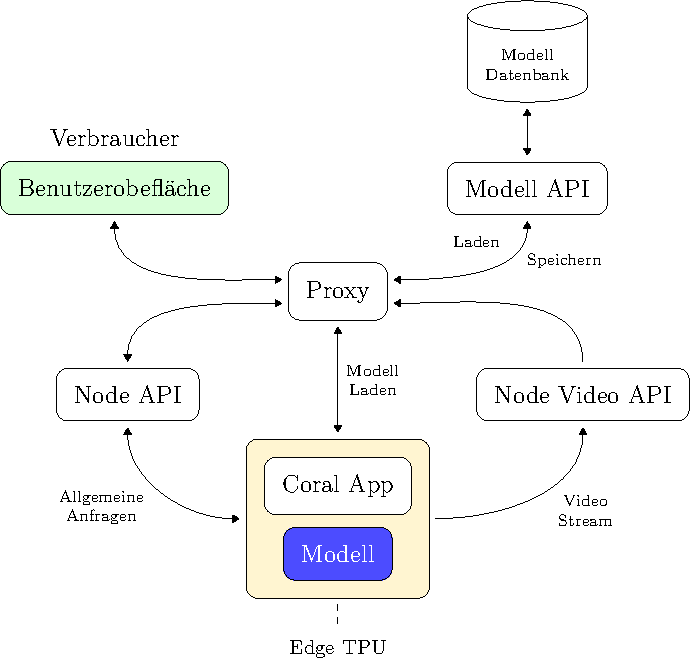
\includegraphics[width=\wLG]{app/app-architecture.pdf}
  \caption{Die Architektur der Anwendung: Ein Modell, das als Dienst
  bereitgestellt wird und verschiedene Services, die mit diesem kommunizieren}
  \label{fig:app-architecture}
\end{figure}

\noindent
Jedes Objekt mit einer Pfeilspitze spiegelt einen Service wieder, insgesamt sind
es sieben Stück. Ein Service ist eine unabhängige, wenn möglich kleine und
unkomplizierte Anwendung, die eine Aufgabe übernimmt.
Um die Verwaltung dieser Services zu erleichtern, wird Docker eingesetzt.
Jeder Dienst kann so isoliert in seinem eigenen Container ausgeführt
und über Docker-Netzwerke verbunden werden.